\chapter{Artificial Neural Networks}

Artificial neural networks are what makes the extension from traditional machine learning models into deep learning methods.

Classification tasks // regression tasks // computer vision and more...

\section{The Architecture of Neural Networks} %-------------SECTION

%---Pathway to Architecture file---
\subfile{Architecture}  


\subsection{More Optimization Algorithms}

With each iteration, after the gradient is computed, a step is taken in that direction.  Yet, just how far a step is to be determined.  If the step is too large, a local minimum may not be found and the algorithm never converge.  If the step is too sall, it may be extremely computationally intensive to reach convergence.  Sometimes, it can be shown mathematically how to determine an optimal step size for special cases \cite{nar2018step}, or several step sizes can be tested \cite{Goodfellow-et-al-2016} and an appropriate one determined.  Other algorithms exist for training neural networks, either as variants to gradient descent or a completely new means; some of which aim to save computation or adjust the step size according to the model.  For example, \textbf{stochastic gradient descent} saves computation by sampling the parameters with which to calculate the gradient.  Other methods like Adagrad (Adaptive Gradient Algorithm), RMSProp (Root Mean Square Propagation), and RProp (Resilient Backpropagation)\cite{rproprprop} aim to adapt the step size rather than maintaining a fixed value for each iteration.

\section{Types of Neural Networks} %-------------SECTION

%---Pathway to Keras_types file---
\subfile{Keras_types}

\begin{comment}
Commenting out the old text, replaced by subfile...

The previous section described a \textbf{Multi-Layer Perceptron} network.  This section is devoted to other network types and their most practical uses. 

Obviously not all types will be covered, but here are a few.  

%\subsection{Multi-Layer Perceptron}
%Keras Model: "sequential"
%This ws described above

\subsection{Convolutional Neural Networks}
Unstructured image data

Convolution operation // Notation // Architecture and diagram

A Convolutional Neural Network (CNN) is a neural network that uses the convolution operation in at least one of its layers \cite{?}.

Convolution operation continuous
$$
C(t) = \int x(\tau)w(t - \tau)d\tau
$$
Convolution operation discrete
$$
C(t) = \sum_{\tau = -\infty}^\infty x(\tau)w(t - \tau)
$$
$x(t)$ is the \textbf{input} and $w(t-\tau)$ is known as the \textbf{kernel}. The shorthand operation for the convolution operation is denoted with an asterisk:
$$
(x * w)(t)
$$

Assumptions for CNN's \cite{Goodfellow-et-al-2016}

\begin{itemize}
  \tightlist
  \item
output is essentially a weighted average  
 \item
$w$ must be a valid probability distribution
 \item
$w$ is 0 for all negative arguments
 \item
values of kernel and input tensors are zero except for the finite set in which values are stored (i.e. size of image)
 \item
 - infinite summation over finite number of array elements
\end{itemize}


\subsubsection{Bird Call Spectrogram example from R}

\textit{(Make brief, include Keras code, stay on track that is is simply an illustration for CNN's)}

Labeled data on recorded bird calls converted into spectrograms of 251x251 pixels.

\begin{figure}[H]
\centering
    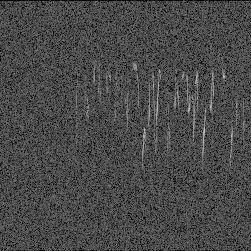
\includegraphics[width = .13\textwidth]{Figures/spectrogramsamps/Cardellina475957.png}
    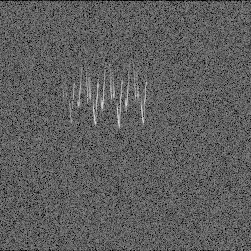
\includegraphics[width = .13\textwidth]{Figures/spectrogramsamps/Geothlypis13687.png}
    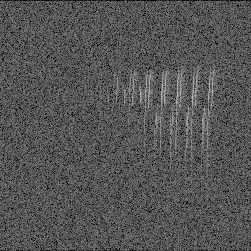
\includegraphics[width = .13\textwidth]{Figures/spectrogramsamps/Seiurus13640.png}
    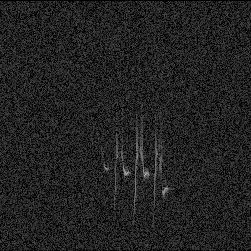
\includegraphics[width = .13\textwidth]{Figures/spectrogramsamps/Setophaga160916.png}
    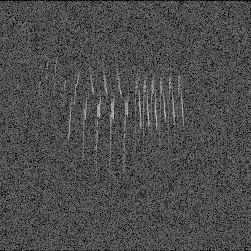
\includegraphics[width = .13\textwidth]{Figures/spectrogramsamps/Spinus192078.png}
    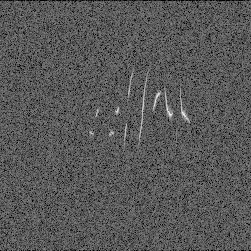
\includegraphics[width = .13\textwidth]{Figures/spectrogramsamps/Spizelloides45125.png}
    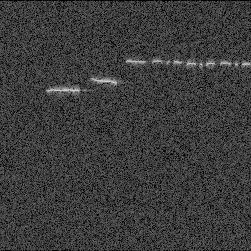
\includegraphics[width = .13\textwidth]{Figures/spectrogramsamps/Zonotrichia139053.png}
\end{figure}

Train the network to be able to identify that bird call based on spectrogram shape.

Use reference: \cite{kahl2017large}

Two-dimensional image $X$ with a two-dimensional kernel $W$
$$
C(i,j) = (X * W)(i,j) = \sum_m \sum_n X(m,n)W(i-m,j-n)
$$

$m$ and $n$ are the representative pixel locations in the relevant dimension, while $i$ and $j$ are the kernel locations, where the convolution is taking place.  The infinite summation is made possible by the fact that values are zero wherever the image is not present.



$$
Insert Example Here
$$

%---POTENTIALLY - make a pathway to the .tex file from RMarkdown ---\subfile{CNN_BCS} 


\subsection{Generative Adversarial Networks}
Unstructured image data

(Notation, no direct coding example)

Image generation to try and fool a "discriminator" network

\subsection{Recurrent Neural Networks}
Unstructured text data

(Notation, MAYBE time series coding example)

NLP/translation/text generation
Time series forecasting

\subsection{Long Short-Term Memory Network}
Unstructured text data

(Notation, no coding example)

\subsection{Convolutional Recurrent Networks}
Unstructured text data

(consider removing)

\end{comment}

\section{Techniques to Improve Model Performance} %-------------SECTION

%---Pathway to performance file---
\subfile{Performance}

\subsection{Example: Tohoku Earthquakes}

%---Pathway to earthquakes_lm_example file---
\subfile{earthquakes_lm_example}

%---Pathway to earthquakes_mlp file---
\subfile{earthquakes_mlp}

